% This line sets the project root file.
% !TEX root = Notes_Gauging_Defects.tex
% !TEX spellcheck = en_US

\subsection{Example: $\Vec(\Z/p\Z)$ bimodules}\label{sec:VecZp-bimodules}

We now list all the $\Vec(\Z/p\Z)$-$\Vec(\Z/p\Z)$ bimodules since we are going to need them in Subsec.~\ref{subsec:VecZ2}. This data is mostly taken from \cite{BBJ19}, and the names assigned to the bimodules are taken from there. Each bimodule $\mathcal{M}$ is labeled by a conjugacy class of subgroups $H\subseteq\Z/p\Z\times\Z/p\Z$ and a $2-$cocycle $\omega\in H^2(H,U(1))$ (see \cite{Etingof2015}). The objects of $\mathcal{M}$ are labeled by cosets of $H$. In general, there are four non-invertible bimodules: 
	\begin{enumerate}
		\item The trivial bimodule $T$, which is coming from the subgroup $\{(0,0)\}$. It has $p^2$ simple objects, which are labeled by the cosets $\{(g,h)\}$ of the group, i.e.\ a simple object in $T$ is $(g,h)$. The left and right action is given as follows
			\begin{equation}
				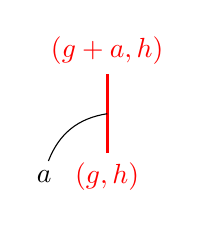
\begin{tikzpicture}[scale=0.8,baseline=(current bounding box.center)]
				\node[red](m) at (0,0) {$(g,h)$};
				\node(b) at (-1,0) {$a$};
				\node[red](abm) at (0,2) {$(g+a,h)$};
				\draw[red,line width=0.4mm] (m)-- (abm);
				\draw (b) to [bend left] (0,1);
				\end{tikzpicture}\hspace{20pt}
				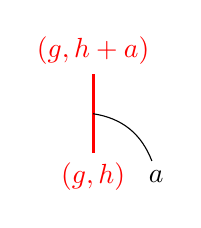
\begin{tikzpicture}[scale=0.8,baseline=(current bounding box.center)]
				\node[red](m) at (0,0) {$(g,h)$};
				\node(b) at (1,0) {$a$};
				\node[red](abm) at (0,2) {$(g,h+a)$};
				\draw[red,line width=0.4mm] (m)-- (abm);
				\draw (b) to [bend right] (0,1);
				\end{tikzpicture}
			\end{equation}
		\noindent
		and the associator for this bimodule is trivial:
			\begin{equation}
				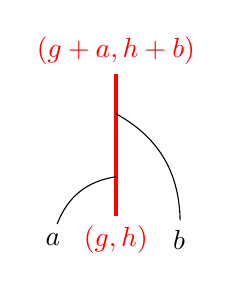
\begin{tikzpicture}[scale=0.8,baseline=(current bounding box.center)]
				\node[red](m) at (0,0) {$(g,h)$};
				\node(a) at (-1,0) {$a$};
				\node(b) at (1,0) {$b$};
				\node[red](abm) at (0,3) {$(g+a,h+b)$};
				\draw[red,line width=0.4mm] (m) -- (abm);
				\draw (a) to [bend left] (0,1);
				\draw (b) to [bend right] (0,2);
				\end{tikzpicture}\ =
				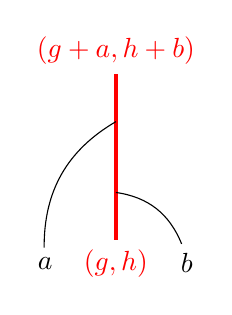
\begin{tikzpicture}[scale=0.9,baseline=(current bounding box.center)]
				\node[red](m) at (0,0) {$(g,h)$};
				\node(a) at (-1,0) {$a$};
				\node(b) at (1,0) {$b$};
				\node[red](abm) at (0,3) {$(g+a,h+b)$};
				\draw[red,line width=0.4mm] (m) -- (abm);
				\draw (b) to [bend right] (0,1);
				\draw (a) to [bend left] (0,2);
				\end{tikzpicture}.
			\end{equation}
		\item The bimodule $L$ from the subgroup $H=\langle(1,0)\rangle\cong \Z/p\Z$, which has $p$ simple objects. The labels are given by the cosets $\{(h,g)|h\in\Z/p\Z\}$, hence the label for a simple object in $L$ is $g$. Left and right action are given by 
			\begin{equation}
				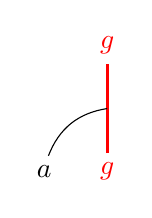
\begin{tikzpicture}[scale=0.8,baseline=(current bounding box.center)]
				\node[red](m) at (0,0) {$g$};
				\node(b) at (-1,0) {$a$};
				\node[red](abm) at (0,2) {$g$};
				\draw[red,line width=0.4mm] (m)-- (abm);
				\draw (b) to [bend left] (0,1);
				\end{tikzpicture}\hspace{20pt}
				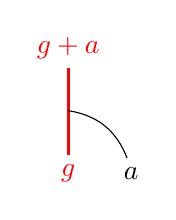
\begin{tikzpicture}[scale=0.8,baseline=(current bounding box.center)]
				\node[red](m) at (0,0) {$g$};
				\node(b) at (1,0) {$a$};
				\node[red](abm) at (0,2) {$g+a$};
				\draw[red,line width=0.4mm] (m)-- (abm);
				\draw (b) to [bend right] (0,1);
				\end{tikzpicture}
			\end{equation}
		and the associator is trivial.
		\item The bimodule $R$ from the subgroup $H=\langle(0,1)\rangle\cong \Z/p\Z$. This bimodule is basically the same as $L$, but in all operations left and right are flipped.
		\item $F_0$, the bimodule from the subgroup $\langle(0,1),(1,0)\rangle\cong\Z/p\Z\times\Z/p\Z$, which has only one object that is denoted $*$. Left and right actions are
			\begin{equation}
				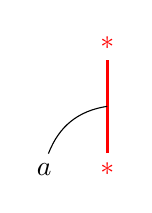
\begin{tikzpicture}[scale=0.8,baseline=(current bounding box.center)]
				\node[red](m) at (0,0) {$*$};
				\node(b) at (-1,0) {$a$};
				\node[red](abm) at (0,2) {$*$};
				\draw[red,line width=0.4mm] (m)-- (abm);
				\draw (b) to [bend left] (0,1);
				\end{tikzpicture}\hspace{20pt}
				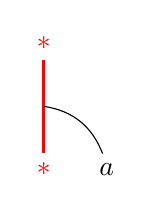
\begin{tikzpicture}[scale=0.8,baseline=(current bounding box.center)]
				\node[red](m) at (0,0) {$*$};
				\node(b) at (1,0) {$a$};
				\node[red](abm) at (0,2) {$*$};
				\draw[red,line width=0.4mm] (m)-- (abm);
				\draw (b) to [bend right] (0,1);
				\end{tikzpicture}
			\end{equation}
		\noindent
		and the associator is trivial.
	\end{enumerate}
Furthermore, there are several invertible bimodules:
	\begin{enumerate}
		\item The bimodule $X_k$, coming from the subgroup $\{(-k,1)\}\cong\Z/p\Z$ with $p$ simple objects. The cosets of this group are $\{n(-k,1)+(h,0)|n\in\Z/p\Z\}$, hence the object labels are $h$. Left and right action is given by 
			\begin{equation}
				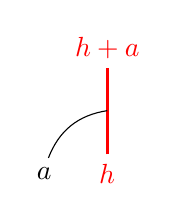
\begin{tikzpicture}[scale=0.8,baseline=(current bounding box.center)]
				\node[red](m) at (0,0) {$h$};
				\node(b) at (-1,0) {$a$};
				\node[red](abm) at (0,2) {$h+a$};
				\draw[red,line width=0.4mm] (m)-- (abm);
				\draw (b) to [bend left] (0,1);
				\end{tikzpicture}\hspace{20pt}
				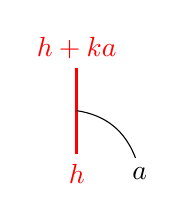
\begin{tikzpicture}[scale=0.8,baseline=(current bounding box.center)]
				\node[red](m) at (0,0) {$h$};
				\node(b) at (1,0) {$a$};
				\node[red](abm) at (0,2) {$h+ka$};
				\draw[red,line width=0.4mm] (m)-- (abm);
				\draw (b) to [bend right] (0,1);
				\end{tikzpicture}
			\end{equation}
		\noindent
		and the associator is again trivial.
		\item The bimodule $F_q$, with $q\in H^2(\Z/p\Z,U(1))\cong\Z/q\Z$. As $F_0$, it comes from the subgroup $\langle(0,1),(1,0)\rangle$ and has only one object denoted $*$. Also, left and right action are defined in the same way as they are in $F_0$, but now the associator is non-trivial:
			\begin{equation}
				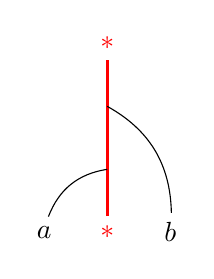
\begin{tikzpicture}[scale=0.8,baseline=(current bounding box.center)]
				\node[red](m) at (0,0) {$*$};
				\node(a) at (-1,0) {$a$};
				\node(b) at (1,0) {$b$};
				\node[red](abm) at (0,3) {$*$};
				\draw[red,line width=0.4mm] (m) -- (abm);
				\draw (a) to [bend left] (0,1);
				\draw (b) to [bend right] (0,2);
				\end{tikzpicture}\ =e^{\frac{2\pi i}{p}qab}
				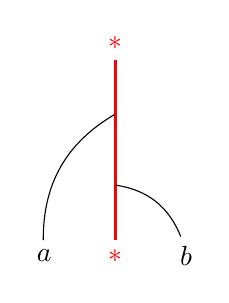
\begin{tikzpicture}[scale=0.9,baseline=(current bounding box.center)]
				\node[red](m) at (0,0) {$*$};
				\node(a) at (-1,0) {$a$};
				\node(b) at (1,0) {$b$};
				\node[red](abm) at (0,3) {$*$};
				\draw[red,line width=0.4mm] (m) -- (abm);
				\draw (b) to [bend right] (0,1);
				\draw (a) to [bend left] (0,2);
				\end{tikzpicture}.
			\end{equation}
		We are especially interested in the $\Vec(\Z/2\Z)$-$\Vec(\Z/2\Z)$ bimodule $F_1$ which we use to introduce defects to a $\Vec(\Z/2\Z)$ spin chain in Sec.~\ref{Ising}. In this case the associator is given by
			\begin{equation}
				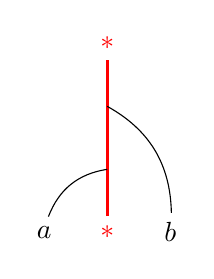
\begin{tikzpicture}[scale=0.8,baseline=(current bounding box.center)]
				\node[red](m) at (0,0) {$*$};
				\node(a) at (-1,0) {$a$};
				\node(b) at (1,0) {$b$};
				\node[red](abm) at (0,3) {$*$};
				\draw[red,line width=0.4mm] (m) -- (abm);
				\draw (a) to [bend left] (0,1);
				\draw (b) to [bend right] (0,2);
				\end{tikzpicture}\ =(-1)^{ab}
				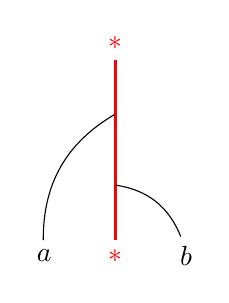
\begin{tikzpicture}[scale=0.9,baseline=(current bounding box.center)]
				\node[red](m) at (0,0) {$*$};
				\node(a) at (-1,0) {$a$};
				\node(b) at (1,0) {$b$};
				\node[red](abm) at (0,3) {$*$};
				\draw[red,line width=0.4mm] (m) -- (abm);
				\draw (b) to [bend right] (0,1);
				\draw (a) to [bend left] (0,2);
				\end{tikzpicture}.\label{eqn:F1}
			\end{equation}
	\end{enumerate}

